\documentclass[12pt]{article}
\usepackage{pdfpages}
\usepackage{eso-pic}
\usepackage{hyperref,url}
\usepackage{graphicx}
\graphicspath{{images/}}
\newcommand\tab[1][1cm]{\hspace*{#1}}

\begin{document}
\begin{titlepage}


%----------------------------------------------------------------------------------------
% TITLE PAGE INFORMATION
%----------------------------------------------------------------------------------------
  \begin{center} % Center everything on the page

  %----------------------------------------------------------------------------------------
  % HEADING SECTIONS
  %----------------------------------------------------------------------------------------
  \textsc{\large Facultatea Calculatoare, Informatica si Microelectronica}\\[0.5cm]
  \textsc{\large Universitatea Tehnica a Moldovei}\\[1.2cm] % Name of your university/college
  \vspace{25 mm}

  \textsc{\Large Medii Interactive de Dezvoltare a Produselor Soft}\\[0.5cm] % Major heading such as course name
  \textsc{\large Lucrarea de laborator\#1}\\[0.5cm] % Minor heading such as course title
  %\textsc{\large Laboratory work}\\[0.5cm] % Minor heading such as course title

\newcommand{\HRule}{\rule{\linewidth}{0.5mm}} % Defines a new command for the horizontal lines, change thickness here

  %----------------------------------------------------------------------------------------
  % TITLE SECTION
  %----------------------------------------------------------------------------------------
  \vspace{10 mm}
  \HRule \\[0.4cm]
  { \LARGE \bfseries Realizarea unui simplu GUI Calculator  }\\[0.4cm] % Title of your document
  \HRule \\[1.5cm]

  %----------------------------------------------------------------------------------------
  % AUTHOR SECTION
  %----------------------------------------------------------------------------------------
      \vspace{30mm}

      \begin{minipage}{0.4\textwidth}
      \begin{flushleft} \large
      \emph{Autor:}\\
      Daniela \textsc{Cazac}
      \end{flushleft}
      \end{minipage}
      ~
      \begin{minipage}{0.4\textwidth}
      \begin{flushright} \large
      \emph{lector asistent:} \\
      Irina \textsc{Cojanu} \\ % Supervisor's Name 
      \emph{lector superior:} \\
      Radu \textsc{Melnic} % Supervisor's Name
      \end{flushright}
      \end{minipage}\\[4cm]

      \vspace{5 mm}
      % If you don't want a supervisor, uncomment the two lines below and remove the section above
      %\Large \emph{Author:}\\
      %John \textsc{Smith}\\[3cm] % Your name

      %----------------------------------------------------------------------------------------
      % DATE SECTION
      %----------------------------------------------------------------------------------------

      %{\large \today}\\[3cm] % Date, change the \today to a set date if you want to be precise

      %----------------------------------------------------------------------------------------
      % LOGO SECTION
      %----------------------------------------------------------------------------------------

      %\includegraphics{red}\\[0.5cm] % Include a department/university logo - this will require the graphicx package

      %----------------------------------------------------------------------------------------

      \vfill % Fill the rest of the page with whitespace
      \end{center}
      
\end{titlepage}
\cleardoublepage

\newpage

\pagenumbering{arabic}
\setcounter{page}{1}
\setcounter{secnumdepth}{4}

\addtocontents{toc}{\protect\thispagestyle{empty}} % no page number on the table of contents page
\cleardoublepage

\section*{Lucrarea de laborator \#3}
\phantomsection

\section{Scopul lucrarii de laborator}
Realizarea unui simplu Web Site personal
Realizarea unui mockup corespunzatorul site-ului care urmeaza a fi realizat
Familiarizarea cu HTML si CSS
\section{Obiective}
Realizarea unui simplu Web Site personal si Mockupul.
Familiarizarea cu HTML si CSS.

\clearpage

\section{Screenshoturi la mockup}

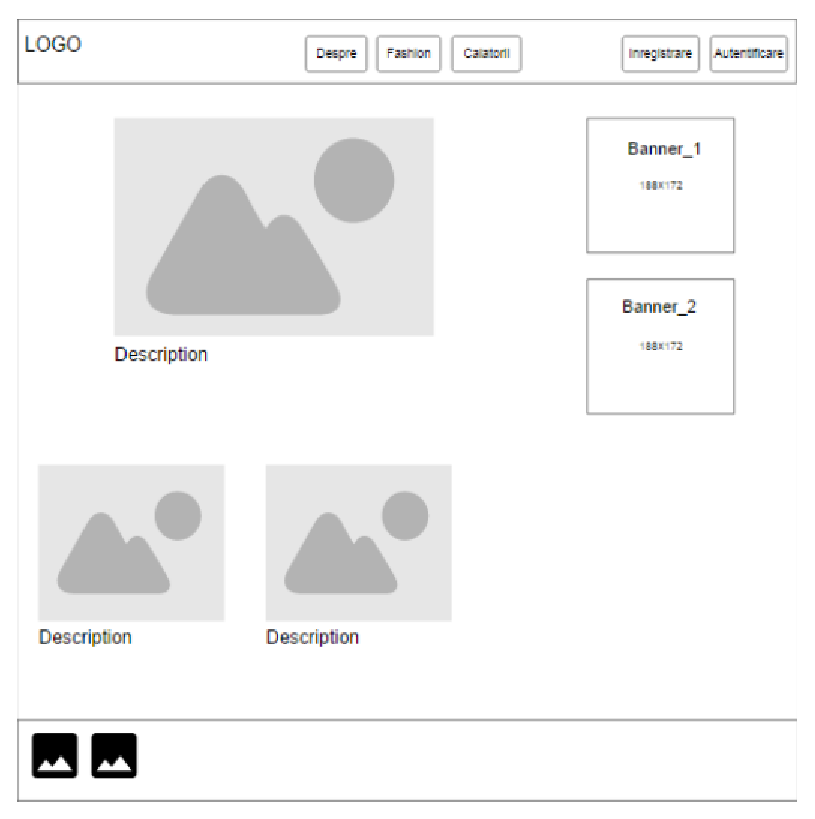
\includegraphics[width=\textwidth]{1.eps}
~\\
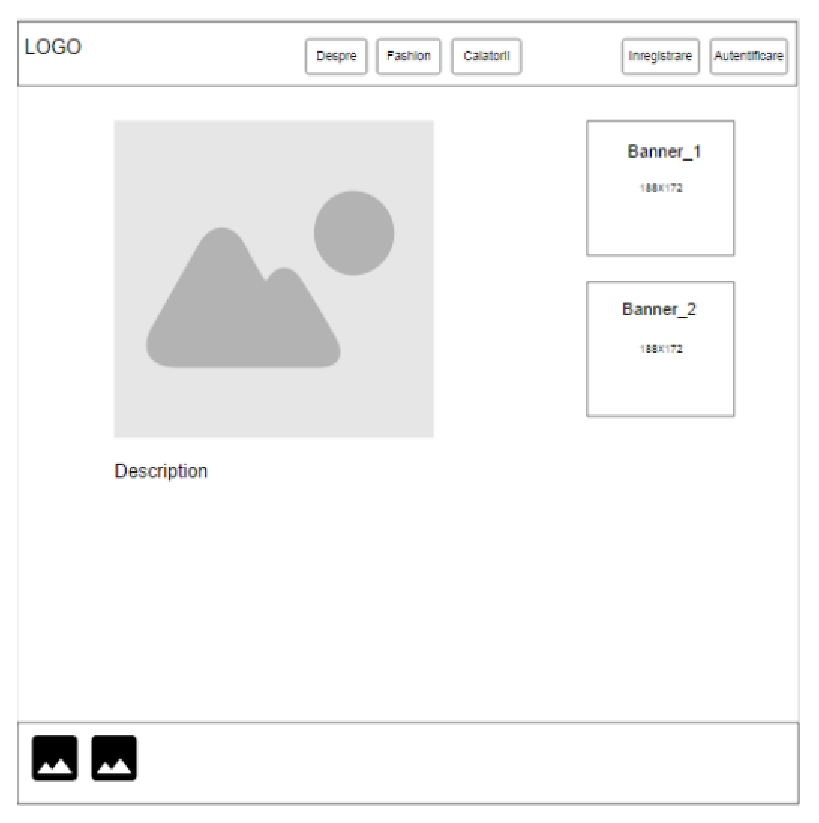
\includegraphics[width=\textwidth]{2.eps}
~\\
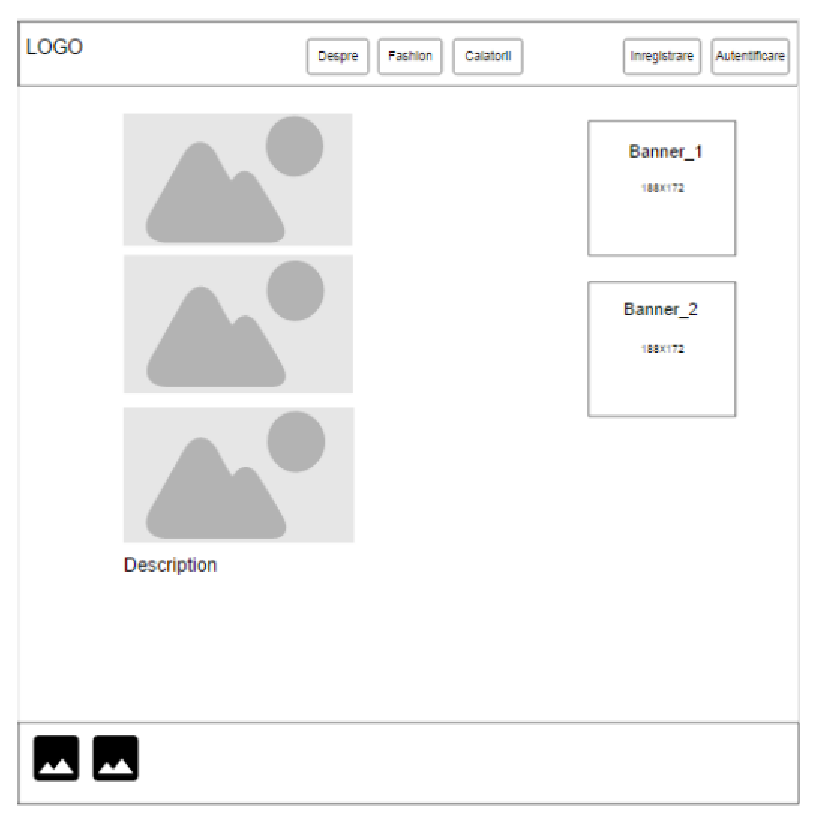
\includegraphics[width=\textwidth]{3.eps}
~\\
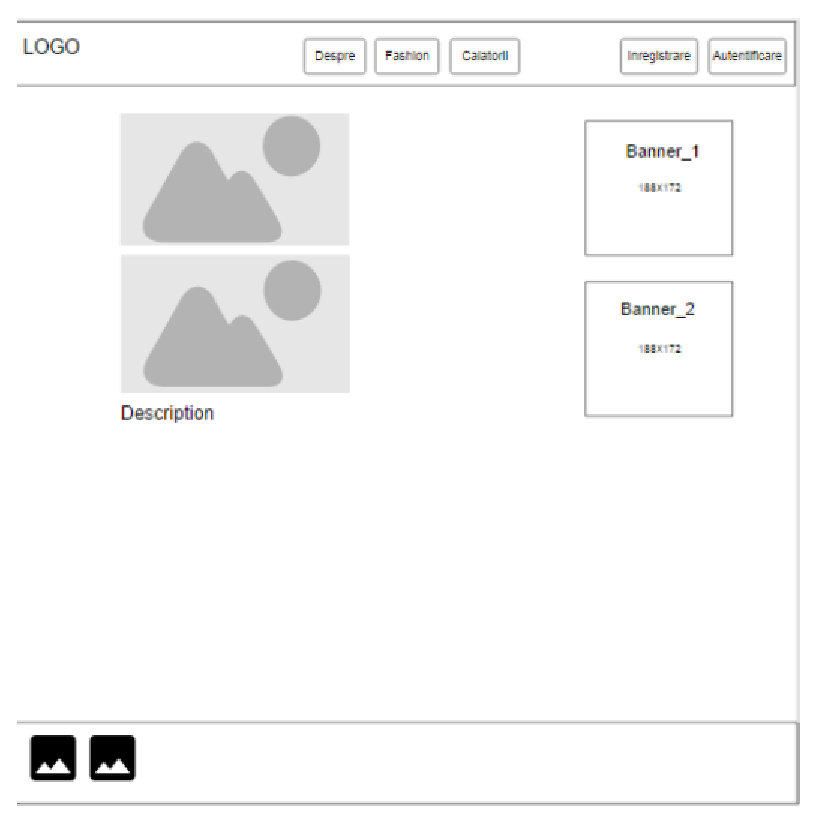
\includegraphics[width=\textwidth]{4.eps}
\clearpage

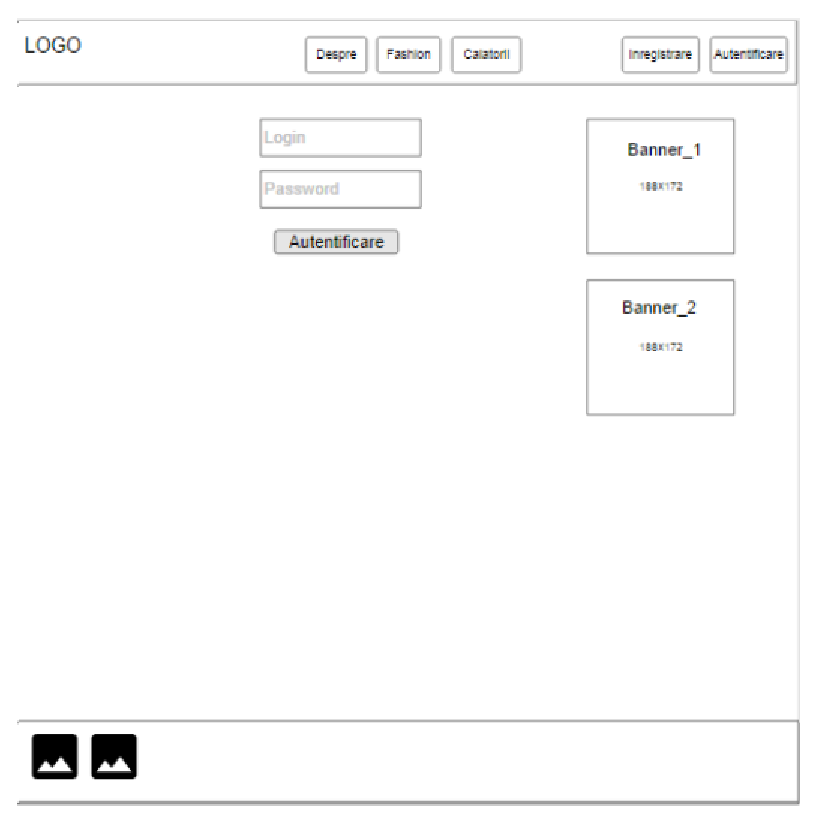
\includegraphics[width=\textwidth]{5.eps}
~\\
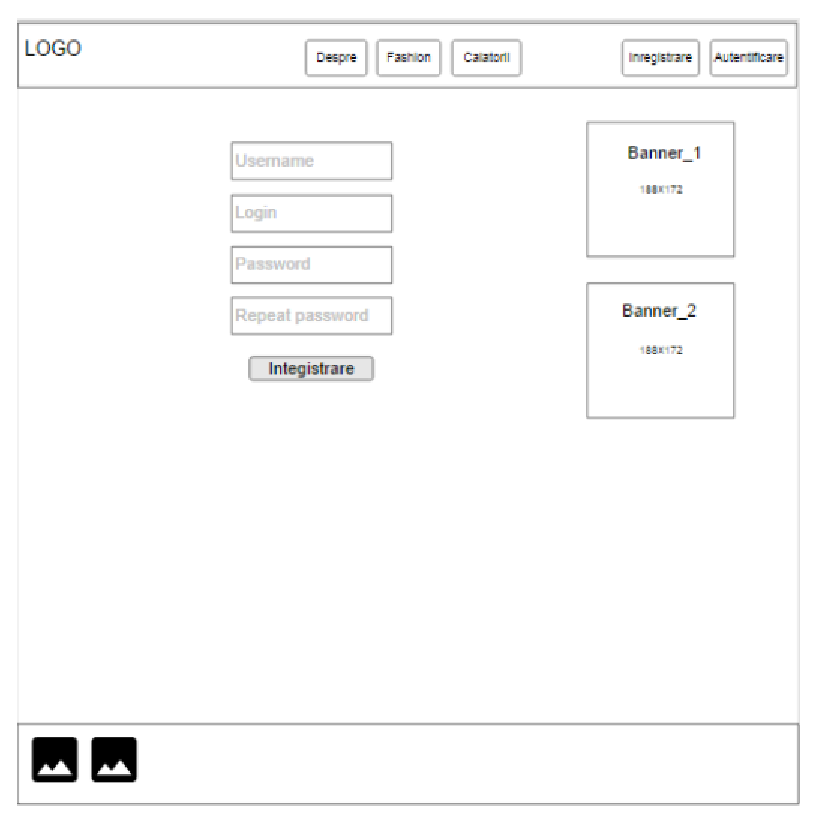
\includegraphics[width=\textwidth]{6.eps}
\clearpage
\section{Concluzie}
In aceasta lucrare de laborator am elaborat propriul web site. Intii de toate am elaborat mockup-ul pentru acest site care reprezinta un schelet si o baza pentru un viitor site si reprezinta un ghid pentru creare functionalitatii site-ului. Text editorul folosit este Notepad++ si limbajele de programare folosite si familiarizate sunt PHP,HTML si CSS. De asemenea am invatat cum sa gestionez pe blocuri site-ul pentru a nu scrie acelasi cod de mai multe ori, dar apelind codul scris o singura data. De asemenea am facut conexiune dintre site-ul creat si cu baza de date , si anume persoanele care se inregistreaza pe site se introduc in baza de date cu datele cu care s-a inregistrat,parola fiind criptata. Web development-ul este interesant prin documentatie, toturiale, si documentare.

\end{document}
